\documentclass[preprint]{aastex}

\usepackage{rotating}
\usepackage{amsmath}
\usepackage{graphicx}
\usepackage{xspace}

\newcommand{\mev}{\text{MeV}\xspace}
\newcommand{\gev}{\text{GeV}\xspace}
\newcommand{\sr}{\text{sr}\xspace}
\newcommand{\s}{\text{s}\xspace}
\newcommand{\ph}{\text{ph}\xspace}
\newcommand{\cm}{\text{cm}\xspace}
\newcommand{\tsext}{\ensuremath{\text{TS}_\text{ext}}\xspace}
\newcommand{\ts}{\text{TS}\xspace}
\newcommand{\pointlike}{{\em pointlike}\xspace}
\newcommand{\gtlike}{{\em gtlike}\xspace}

\shorttitle{Search for Extended LAT Sources}

\begin{document}

\title{Search for Spatially Extended Fermi-LAT Sources Using Two Years of Flight
Data}

\author{
J.~Lande\altaffilmark{3}, 
\altaffiltext{3}{W. W. Hansen Experimental Physics Laboratory, Kavli Institute for Particle Astrophysics and Cosmology, Department of Physics and SLAC National Accelerator Laboratory, Stanford University, Stanford, CA 94305, USA}
}


\begin{abstract}
We present a new method for analyzing spatially extended sources with
the Fermi Large Area Telescope (LAT), the primary science instrument
on the {\em Fermi Gamma-ray Space Telescope (Fermi)}.  We provide a
series of Monte Carlo studies that were done to validate this tool.
We then calculate the Fermi LAT's sensitivity to spatially exnteded
sources.
We then apply this tool to test all sources in the 2FGL Two Year Catalog
for extension.\cite{2FGL} We then report on the discovery of XXX new
extended sources.
\end{abstract}

\section{Introduction}

% * Resolving spatially extended Fermi sources is important for 
%    * studying supernova remnants, 
%    * pulsar wind nebulae, 
%    * galaxies,  
%    * potentially dark matter or new physics.
% * We searched all 2FGL catalog sources
% * Systematic test for a certain kind of (~ small) regularly shaped extended 

The Large Area Telescope (LAT) is a pair conversion telescope on the
Fermi Gamma-Ray Space Telescope that has been surveying the gamma ray
sky since June 2008.  Fermi is particuarly well suited for surveying
the entire Gamma-ray sky since it has a broad energy coverage ($20\mev$
and $300\gev$), a wide field of view ($\sim 2.4 \sr$) and large effective area
($\sim 8000 \cm^2$ at $>1\gev$).

The LAT has been essential in understanding a variety of astrophysical
sources including Active Galactic Nuclei, Pulsars, and Supernova Remnants.
Many of the astrophysical sources seen by the Fermi LAT, espeically
galactic Supernova Remnants and Pulsar Wind Nebulae, can be resolved at
other wavelengths and could potentially be resolved by the LAT.

studying supernova remnants, 
pulsar wind nebulae, 
galaxies,  galaxy clusters, and potentially dark matter and new physics.


Resolving spatially extended $\gev$ sources is important for studying a
variety of science topics. The most important use of spatial morphology
is in source identification. Many of the sources found in $\gev$ sources

Nevertheless, morphological studies of sources in the $\gev$ energy range using
the Fermi LAT is challenging primarily because of the significantly energy
dependent PSF and because of systematic errors in the
galactic diffuse emission. The Fermi PSF varies from over $XXXXX^\circ$
at $100\mev$ to $XXXXX^\circ$ at $100\gev$ and so the higher energy photons are

The Large Area Telescope (LAT) on the Fermi Gamma-Ray Space Telescope
has been surveying the Gamma-ray sky since August 2008. The LAT has been
been essential in studying a variety of astrophysical sources including
Active Galactic Nuclie, Pulsars, Supernova Remnants. 
One of the important data productes 

Using 11 months of data, the LAT produced the best-resolved survey of the sky
in the $100\mev$ to $100\gev$ energy range\cite{2FGL Paper}. The


\section{Analysis Method}


%   * Difficulty of studying spatially extended sources
%   * Pointlike, great features
%   * modifying it to fit spatially extended sources.
%      * semi-analytic convolution formula
%   * importance of fitting position + extension + spectrum simultaneously to apply statistical significance
%   * Monte Carlo Validation
%

Performing morphological studies of sources in the $\gev$ energy range using
the Fermi LAT is challenging primarily because of the significantly energy
dependent PSF and because of systematic errors in the
galactic diffuse emission. The Fermi PSF varies from over $XXXXX^\circ$
at $100\mev$ to $XXXXX^\circ$ at $100\gev$ and so the higher energy photons are
significantly more important for studying the shape of sources. One could
ideally look just at the highest energy photons, but the trade off is that
for typical sources many more source events are expected at low energy.
For this reason, it is especially important to use as much of the data
as possible.

The second primary difficult in studying spatially extended sources is
systematic uncertainties in the diffuse emission. Systematic errors are
notoriously difficult and will be discussed more later, but the important
point to make here is that one of the most important diagnostic tools for
studying systematic errors is being able to iterate the analysis while
varying different parameters such as what goes into the diffuse model.

A new analysis tool has been developed to address these unique
requirements for studying spatially extended sources with the Fermi
LAT. The overall approach for this analysis is to perform a maximum
likelihood analysis where the Poisson likelihood for observing the
measured counts is computed given an assumed sky model. The parameters
of the sky model are then fit by maximizing the log of the likelihood.
To study the extension of a source, one can assume a particular shape
for an extended source (e.g. a disk or Gaussian), and fit the spatial
parameters of that source.

In principle, the entire task can be done using the standard science
tools package \gtlike\cite{Science-Tools-gtlike}. But \gtlike is
only able to fit the spectral parameters of the source, so the extension
fitting would have to be done as an external loop. Typically, the run time
for a binned source analysis using \gtlike is several hours so this loop
would be especially time consuming. In principle, parallel computing could
ease this burdon, but parallel fitting algorithms are rather untested
and complex. Furthermore, the machinery required to do something like
this would necessarily be rather complex. What has typically been done by
the Fermi team to study extended sources is to fix the assumed position
of the extended source, either by our knowledge of a source from other
wavelenghts, or by fitting it as a point source. Then, a profile of the
likelihood as a function of extension is developed using \gtlike
and the maximum of this profile. This approach is not optimal because it
needs not be the case that the best fit position of a point source would
be the same as the best fit position of an extended source. Furthermore,
by not fully maximizing the likelihood, this method is not as significant to
extension, especially of faint sources. And finally, since this approach
is so computationally intensive, no large scale Monte Carlo effort has been
launched to validate the method.

Instead, an alternate approach was developed for performing
a morphological analysis. An alternate maximum likelihood fitting
package called \pointlike has been developed by the Fermi
collaboration and we have expanded its functionality to fully support
analyzing spatially extended sources. \pointlike is most thoroughly
described in Matthew Kerr's Ph.D Thesis\cite{Matthew_kerr_phd_thesis}
but the important aspects will be summarized below. What differentiates
\pointlike most significantly from \gtlike is its emphasis
on speed by introducing approximations into the calculation of the
likelihood function while at the same time trying to reduce any
numerical errors that may be introduced.  Like binned \gtlike,
\pointlike bins the sky both in position and energy.  Unlike 
\gtlike, \pointlike relies on the {\em healpix} representation of spatial
bins\cite{healpix_paper} and scales the size of each spatial bin to be
smaller than the PSF. This is convenient because it no
significant information is lost due to binning at all energies and it is
always a good approximation that the model predicted counts are uniform
across a spatial bin. 
\pointlike additionaly bins the Fermi Gamma-rays by their conversion type,
which corresponds to whether the photon converted in the front or back
part of the detector. Since the PSF is smaller for front entering events,
one would expect binning each conversion type independently to improve
our sensitivity.
Furthermore, \pointlike uses a sparse matrix
representation of the spatial bins where only the bins with counts in them
are looped over. The only downside to this is that the integral of the
model predicted counts must be independently calculated.  Effectively,
\pointlike efficiently interpolates from a totally binned analysis
at low energy (where the resolution is poor and there are many counts)
to an unbinned analysis at high energy (where the resolution is very
good but there are few counts). This approach provides a significant
savings in time while introducing only small numerical error.

We have modified \pointlike to support fitting spatially extended
sources.  To do this, we introduced a new class of diffuse sources where
the spatial and spectral information completely decouple and where
the spatial shape is parameters by simple objects (Disks, Gaussian).
The code consistently convolves the extended source shape with the point
spread function (as a function of energy) and integrates the spectrum over energy
to computed model predicted counts.

Finally, \pointlike allows the spatial parameters of an extended
source to be simulataneoulsy fit. \pointlike uses the Minuit fitting
library to perform the maximum likelihood maximization of the position
and extension of an extended source\cite{Minuit reference}.  At each
step in the fit of the shape, the spectral parameters of the entire sky
model are reoptimized. To avoid projection effects, what is directly
fit is not the longitude and latitude of the source but instead
the displacement in a rotated reference frame. The covariance matrix is
then computed and inverted to estimate the statistical errors on the
position and extension.

\pointlike optimizes the analysis of extended sources in two ways.
First, for extended sources which are radially symmetric, the convolution
of the source shape with our parameterization of the PSF can be performed
semi-analytically. Generally, at a given energy the observed 
photon distribution is
\begin{equation}
  \text{PDF}(\vec r) = \int  \text{PSF}(|\vec r - \vec r'|)I_\text{src}(\vec r') d A' 
\end{equation}
where $I_\text{src}$ is the extended soruce shape and the PSF is parameterized by
\begin{equation}
  \text{PSF}(\vec r) = 
  \frac{1}{2\pi\sigma^2}
  \left(1-\frac{1}{\gamma}\right)
  \left(1+\frac{u}{\gamma}\right)^{-\gamma}
\end{equation}
Here, $\sigma$ and $\gamma$ are parameterize the $PSF$.
If the extended source is radially symmetric, then
$I_\text{src} (\vec r') = I_\text{src} (r')$ and the angular part of the
integral can be done analytically, leaving a simpler one dimensional
integral:
\begin{equation}
  \text{PDF}(u)= \int_0^\infty dv
  I_\text{src}(v) 
  \left(\frac{\gamma-1}{\gamma}\right)
  \left( \frac{\gamma}{\gamma + u + v}\right)^\gamma 
  \times ~_2F_1 \left(\gamma/2,\frac{1+\gamma}{2},1,\frac{4uv}{(\gamma+u+v)^2}\right)
\end{equation}
Not only is this convolution formula faster, but it has the advantage
that it more accurately reduces to the actual PSF shape as the source's
size decreases.  Decreasing the numerical difference between a small extended
source and the PSF is important when searching for smaller extended sources
and when determining the statistical significance of a detection.

There is one final approximation which speeds up the convolution.
Generally, the PSF is a function of the angle $\theta$ of the incident
event measured relative to the normal to the LAT. To avoid repeatedly
convolving the source shape with the PSF at a series of $\theta$ angles,
an effective PSF is fit to the weighted sum of the PSF times the exposure
at different $\theta$ angles.  Since the source convolution has to be
done at each fit iteration, these optimization were essential for making
this tool fast enough for the following analysis. Typically, the entire
process of fitting the extension and estimating the errors for a source
would run on the order of an hour.

To calculate the statistical significance of the extension of a source,
one can define a parameter $\tsext$ as twice the increase
in log likelihood between fitting a source with a
spatially extended hypothesis and a point hypothesis. 
So $\tsext=2\times(LL_\text{ext}-LL_\text{ps})$.

In going from fitting a point source to fitting a simple extended source such as
a disk, the source's width is the only degree of freedom added to the model. According to
Wilk's Theorem, the distribution of $\tsext$ for no signal (when there is a true
point source) should follow a $\chi^2_1$ distribution with one degree of freedom\cite{Wilks_Theorem}.
Wilk's Theorem only holds when the likelihood is maximized simultaneoulsy
fitting all of the parameters of model. It is for this reason why 
\pointlike
goes through such great effort to simultaneously fit the position, extension,
and spectral paramters of a source.

On the other hand, since the null hypothesis rests on the edge of
parameter space, when the extension is fixed to 0, Wilk's Theorem does
not formally hold\cite{Warnings about Wilk's Theorem Paper}.  One might
expect the actual distribution to be a half $\chi^2_1$ distribution with
one degree of freedom plus half of a delta function at 0:
\begin{equation}
  P(\ts)=\tfrac{1}{2}(\chi^2_1(\ts)+\delta(\ts)).
\end{equation}
The false detection probability can be estimated by integrating this function 
from an observed test statistic value to infinity. It is for this
particular distribution that the often quoted result holds that
$\sqrt{\ts}$ is a measure of the number of $\sigma$ of the detection.

The half $\chi^2_1$ distribution was found by a monte carlo study
to hold for the special case of source finding of EGRET sources using the
maximum likelihood technique.  They were comparing the hypothesis of a
source to the hypothesis of just a background\cite{Mattox_et_All_Paper}.
Their argument for why this null hypothesis distribution was reasonable
was that half of the time, statistical underfluctuations would cause
there to be fewer fewer photons then expected where the sources is being
tested. Since the maximim likelihood machinery cannot fit negative
sources (which would lead to negative model predicted for which the
poisson likelihood is undefined), half of the tests would not have the
likelihood improved by adding a source to the model and $\ts=0$.
It is for the case that the null distribution has 

It seems plausable that a similar situation could happen for when testing
a source for extension. Half of the time, statistical flucutations might
make the observed counts narrower thant the point spread function and
the likelhood would not improve by fitting the source with an extended
hypothesis. We tested this hypothesis below using a dedicated monte
carlo study.

One issue that we found when testing this analysis method is that
despite our best efforts, there was always a small discrepancy between
the likelihood value when fitting the source as a point source and when
fitting it as an extended source with a small extension.  This is to be
expected due to numerical innacuracies introduced by the convolution.
For most cases, this error is insignificant. It would not significanlty
bias any of the fit values or errors. But it would bias the distribution
of $\tsext$ in the null hypothesis. To correct for this,
instead of computing the likelihood in the null hypothesis by fitting
a point source, a new source model was introduced which is an extended
source with its extension fixed to a very small value. $LL_\text{ps}$
is then calculated by refitting this source using the same extended
source fitting code. It was only after introducing this change that we
were able to get broad agreement between simulations and Wilk's theorem.

\section{Monte Carlo Validation}\label{monte_carlo_validation}

We performed a dedicated monte carlo study to validate \pointlike for
studying spatially extended sources and also to demonstrate that we can
use $\tsext$ as a test of the statistical significance
of a source's extension.  The monte carlo study involved simulating point
sources of varying spectral models on top of a simulated background. The
simulated point source was then fit using \pointlike as both an extended
source and a point source and $\tsext$ was calculated.

Fermi LAT data was simulated using the publically avaliabable Science
Tools package {\em gtobssim}\cite{GTOBSSIM_CITATION}. The sources were
simulated with a powerlaw spectral model with 6 Were given 6 $>100\mev$
fluxes ranging from $3\times 10^{-9} \ph/\cm^2/s$ to 
$10^{-6} \ph/\cm^2/s$.
The sources were then simulated with spectral index ($\gamma$) values of
1.5, 2, 2.5, and 3.  These values were picked to probe a representative
range measurable values.  For particular spectral indices, only the
fluxes which would create a statistically significant source detection
($\ts>25$) where selected, since we are only interested in
testing for extension sources with a significant extent. The sources were
simulated on top of an isotropic powerlaw background with a Sreekumar-like
spectrum ($>100\mev$ flux of 1.5e-5 and spectral index 2.1).\cite{Sreekumar
et al. ApJ 494 pag 523 1998}

The monte carlo simulation was perforormed over a one year time interval using
a default rocking profile and an assumed livetime fraction of 0.8.
The reconstruction was perfromed with events from an energy range of
$1\gev$ to $100\gev$ using 4 energy bins per decade and using the Pass 7 Version 6
source instrument response function (IRFs) to be consistent with the following analysis.

For most of the spectral models, over 10,000 statistically independent simulations were performed.
For fainter sources, some of the simulated sources, statistical flucatuations
caused the source to be not significant and they were excluded from the following analysis.
Table~\ref{ts_ext_num_sims} shows the parametesr used in the simualtion,
the number of simulations perfromed, and the average test statistic value.


The results of the monte carlo simulation are shown in
figure~\ref{ts_ext_mc}.  The cumulative density function (CDF) is plotted
against $\tsext$ For reference, the CDF for $\chi^2_1/2$,
suggested by Wilk's Theorem, is also plotted for comparison. Overall,
there is good agreement between Wilk's theorem, although the agreement
is not perfect.  Possible reasons for departure from Wilk's theorem may
include \pointlike ignoring energy dispersion, which would generally change
the shape as a function of energy, numerical innacuracies in evaluating
the convolution algorithm, or possibly problems with the fitting algorithm
getting stuck in false minimum. It is important to emphasize that if
our emperical curve lies to the left of the curve we assume to estimate
significance, we would underestimate the statistical significance of
our result. Since this is the case for most of our simluations, we are
reasonable confident that $\sqrt{\tsext}$ can be safely
used as a measure of the statistical significance of a source's extension.

\section{Extended Source Sensitivity}

We performed another monte carlo study to determine the Fermi LAT's
sensitivity to spatially extended sources. The sensitivity to extension
is defined as the flux at which 
the average value of $\tsext$ for a source is 
e equal to 25 (for a given spectral model). This correseoncs
to an average extension significance of $5\sigma$.  This is not the
sensitivity to detect an extended source but instead the sensitivity to
resolve an already detected source as being extended.  

One would intuitivly expect that we would be less sensitivie to resolving
small extended sources since they would be lost in the PSF.  Similarly,
we would be less sensitive to very large extended sources which would
get completely lost in the background. Furtheremore, one expects our
sensitivity to be greater for harder sources since our angular resolution
improves significantly with energy.

To calculate the LAT's sensitivity to spatially extended sources,
we simulated sources with a uniform radially symmetric
disk morphology on top of a powerlaw
Sreekumar-like isotropic spectrum.\cite{Sreekumar et al. ApJ 494 pag
523 1998}.  For a given extension and spectral index, we calculated the
sensitivity by varying the flux of a source until we found 
when $\tsext=25$. In particular, we hand picked a flux range
where $\tsext<25$ and $\tsext>25$ and simulated 10 points with
a log uniform distribution in this range and performed an extension
test for each of these fluxes. Since the measured signifciance is
a statistical which will vary from realization to realization,
we then repeated this procedure $>15$ times for each spectral
and spatial model.
By fitting a line to the flux vs $\tsext$ data, we were able to
estimage the flux at which $\tsext=25$.

Our first result is the extension sensitivity for sources of varying
spectral indices. The result is shown in figure~\ref{index_sensitivity}.
We computed the sensitivty for sources with a spectral index of 1.5,
2, 2.5, and 3 and for sources of 20 extensions varying from $0.1^\circ$
to $2.0^\circ$. The $y$ axis is the $100\mev$ to $100\gev$ flux of the
source and the $x$ axis is the monte carlo extension. The curves then
represent the division in this extension and flux space where one gets
on average $\tsext=25$.
The solid lines of the plot are the sensitivity computed when using
with all events from $100\mev$ to $100\gev$. The dashed lines is the
same sensitivity but only using events from from $1\gev$ to $100\gev$.

This results shows that our extension sensitivity is
significantly better for harder sources where there are more high
energy events. Furthermore, our sensitivity is best for sources with an
extension around $0.5^\circ$.  our sensitivity gets significantly worse
for very small sources and gets slightly worse for very large sources.

Futheremore, we note that except for the hardest or largest sources,
our sensitivity is almost entirly whether or not we use events from
$100\mev$ to $1\gev$. On the other hand, other systematic errors become
increasingly important at low energy so for our extension search we will
not use the events in this energy range.

We performed a second computation to see how the LAT's extension
sensitivity varied with increasing background, as is at lower latitude
in the galactic plane. To do so, we computed the sensitivity using the
extragalactic barground as well as 10 and 100 times the extragalactic
background. The latter result approximatly represents the intensity of
the galactic diffuse emission near the galactic center. The results are
shown in figure~\ref{diff_factor_sensitivity}. Two plots are presented,
one fitting only in the energy range between $1\gev$ and $100\gev$ and
one fitting only in the energy range between $10\gev$ and $100\gev$. For
each plot, the $y$ axis quotes the flux in the fit energy range and the
simulation was done only for a representivite spectral index 2 source.

These plots show that we are much less sensitivie to extended sources in
a higher background region. By comparing the two plots, we also see that
we would be more sensitive to an extended source if it had the same
integral flux, but only over a higher energy range. This is 
consistent with the improved angular resolution at higher energy.

\section{Extension search method}

The LAT two year catalog presented a search for all
statistically significant sources that are detected in the $\gev$
sky\cite{2FGL_catalog}.  The catalog group's source finding method assumes
that the emission originated as point sources and what was presented was
a list of all sources fit assuming a point source spatial hyopthesis. All
published extended sources were modeled by the catalog group as extended
sources, but no attempt was made to test if other sources in the catalog
could be spatially resolved.

We performed a search of all Fermi sources found in the second Fermi LAT
catalog for extension.  We performed the extension fit using \pointlike.
To perform this search, we built a model of the sky consistent with
the two year catalog's model.   We used the same two year data set and
the same pass 7 instrument response function We used the same galactic
diffuse, isotropic diffuse, and earth limb emission model. The spectrum
of the galactic and isotropic diffuse models were refit during the
analysis. The earth limb emission was fixed to predicted value.

For each source, we used a circular $10^\circ$ region of interest centered
on our source. We performed a fully binned analysis.  The spatial bin
size was scaled with energy as was described above and we uniformly
binned in log energy, using 4 binned per logarithmic decade of of energy.
We included all background catalog sources within $15^\circ$ of the source
of interest and refit the spectral parameters of sources within $2^\circ$
of our source.

As was shown, we gain very little in sensitivity using events with energy
below $1\gev$. On the other hand, the large PSF at low energy makes us
more succeptable to systmetic errors arising from source confusion and
from out modeling of the galactic diffuse emission.  For that reason,
we performed our search using events between $1\gev$ and $100\gev$.

We also performed a search for extended sources using events only between
$10\gev$ and $100\gev$. Even though we are testing the same sources,
this approach is complimentary because there are regions in the galactic
plane where at lower energies the diffuse emission dominates and is
likely not perfectly modeled. On the other hand, at the highest energies
accessible by the LAT, the galactic diffuse emission will be smaller and
we might expect to detect significantly harder soruces. This approach
of using only events above $10\gev$ was succesfully used to detecting
HESS J1825-137 with the Fermi LAT~\cite{HESS J1825 paper}.

For each source we were testing, we modified the source to have a
uniform radially symmetric disk spatial shape and then used \pointlike to
simultenously fit the position and extension of the source. As described
above, we additionally modified the source to be a extended source with
it's extension fixed to $10^{-10\circ}$ and fit this position of this
pseudo source. For each source, we then computed the increase in log
likelihood fitting with the extended hypothesis and looked at all of
the sources with $\tsext>16$ corresponding to a $4\sigma$ statistical
significance of extension.

We expect most extended sources to be galactic sources since
extragalacitc sources are typically too far away to be spatially
resolved. Unfortuantly, the galactic plane is the most difficult place
to find sources since they must be found for on top of the anisotropic
galactic diffuse emission.  Modeling the galactic diffuse emision is
very difficult~\ref{first_diffuse_paper}.  And finding sources in the
galactic plane is notoriusly difficult, as was discussed in the Fermi
catalog~\ref{1FGL}. One would expect extended sources to be even more
difficult to detect since diffuse emission residuals are expected
to be large compared to the PSF. Furthermore, the galacitc plane
is very crowded and there is a degenecy between an extended source
and multiple point sources. So finding a source with
$\tsext>16$ is not sufficint for detecting an extended.

For each of the extended source candidates for which either the analysis
using events above $1\gev$ or $10\gev$ found $\tsext>16$
and performed several followup analyses to substantiate our analysis.

First, we took the spatial and spectral model found using \pointlike
and performed a crosscheck by refitting the spectral parameters using 
\gtlike.
We used a square ROI $10^\circ$ in diamater, the same 4 degrees
per decade, and $0.125^\circ$ energy binning.
The \gtlike analysis provided a second estimate of the spectral
paramters of the extended source as well as a second calculation of
$\ts_\text{disk}$, $\ts_\text{point}$, and 
$\tsext$. We only looked for extended sources which 
both \pointlike and \gtlike considered significantly extended.

Additionaly, we generated for each 
extended source candidate residual test statistic maps. 
The residual TS Map

Large
TS values in test 


We generated a residual test statistic maps to look for
, which is a map of the test
statistic adding new points
Figure~\ref{res_tsmaps} shows an example residual TS map.






\section{Validation of Known Extended Sources}
\label{validate_known}

We validated our method by testing for extension all of the sources
which the Fermi Collaboration had previously published on.  We applied
no special method to test these sources but used the same pipeline which
was used to test all other catalog sources.  The results are published
in table~\ref{known_extended_sources}.  Using events with energies
greater than $1\gev$, our analysis succesfully fit the extension of the
the two galaxies the Large Magalengic Cloud and the Small Magalenic
Cloud.~\cite{SMC & LMC Paper}.  Our tool also successfully detected the
extension of hte supernova remenants IC443, W28, W30, W44, and W51C.

Using events above $10\gev$, we were able to succesffuly fit the extesion
of HESS J1825-137\cite{HESS 1825 paper}. Our analysis of MSH 15-52 using
events above $10\gev$ found an extension consistent with the publisehed
result, but with $\tsext=11.2$.\cite{MSH 15-52 Paper}. This
is most likely because the published analysis used events above $6\gev$.

Our analysis failed to detect the extension of Vela X. Vela X can only be
successfully analyzed after applying a phase cut to removed the heavily
dominant emission from the pular.

Our analysis also failed to detect a significant extension for the
Centaurus A Lobes.\cite{CenA paper}. This is most likely because the
discoverd emission was significantly more complicted then a uniform
radially symmetric Disk.  Furthermore, our analysis failed to correctly
fit the extension of the Cygnus Loop\cite{Cygnus Loop Paper}.  This is
most likely because Cygnus Loop is rather large and its shell type
morphology is not well represented by a uniform disk. The source is
also rather soft so the publisehd results used a larger energy range
then our search.


The difficulty our analysis analysis had fitting the extension of several
of the already published extended sources should be used to emphasize
the difficultly with which

\section{Test of 1LAC Sources}

To validate our method and assess systematic issues with our
analysis, we used \pointlike to test known active galaxies (AGN) for extension.
\gev emission from AGN is believed to comes from the
core of supermassive blackholes. Since this happens in a very small region
in the core of very distant galaxies,

AGN are not expected to be spatially resolvable and therefore
provide a good calibration source to demonstrate the efficacy of our
tool. Nevertheless, it would be very interesting if AGN could be
spatially resolved AGN and there are theories that predict
this\cite{pair_halo_paper, http://adsabs.harvard.edu/doi/10.1086/187222}.

Following the Fermi-LAT one year catalog, the Fermi collaboration
published a list of the Fermi catalog sources that had a high probability
association with AGN. The first year catalog had 709 AGN associated with
671 distinct 1FGL sources at high latitude ($|b|>10^\circ$).  For our
study, we are looking to assess systematics with extension fitting so
it is important to avoid any possible issues with AGN associations.
For that reason, we select only the 599 AGN which make it into the
``clean'' AGN sample. An AGN association is only considered ``clean''
if it has a high probability of association $P\ge 80\%$, if it is the
only AGN associated with the 1FGL source, and if there are no flags
on the source which shed doubt on the source\cite{1FGL}. These last two
conditions are especially important for our analysis. One might expect
source confusion between two AGN look like a spatially extended source.
Testing only unflagged sources is also important because it removes
any catalog sources coincident with structures in the diffuse emission.
It is possible that these flagged catalog sources which are really poorly
modeled diffuse emission might also look extended.

Of the 599 ``clean'' AGN, we select 556 of these 1FGL sources which
we uniquely associate with a 2 year catalog source. And we furthermore
restrict our select to 515 of these AGN for which we fit $\ts>25$ using
\pointlike.  Our intention here is not to find the largest sample of
AGN and this will be the scope of a follow up AGN association paper. Our
purpose is simply to find a good sample of AGN which can be used to
test the systematics of our tool.

Using the same extension fitting procedure as described above, we test
these 515 AGN for extension. A histogram of the fit \tsext values is
shown in figure~\ref{agn_ts_ext}. Overlaid on the plot is again
a $\chi^2/2$ distribution suggested by Wilk's Theorem.
This plot shows a worse agreement with the theoretical distribution
then was found by our monte carlo study in figure~\ref{ts_ext_mc}. 

Several possible systematics could cause this discrepancy. The first
is that in our analysis we fit each source with a powerlaw index.
AGN tend to have curved spectral and fitting with a wrong spectral
model might effect the value of \tsext. Nevertheless, since we use only
events with $E>1\gev$, this would effect is not expected to be large.
Another possible source for the discrepancy is that pointlike performs a
likelihood analysis without modeling the energy dispersion of our source.
But energy dispersion is expected to be more significant at low
energy and furthermore if this was a signifciant effect the same results
would have showed up with the monte carlo simultions which included the
effects of energy dispersion. 

The third possible effect causing this discrepancy is an
imperfect modeling of the PSF of the LAT.  Before launch,
the LAT PSF was determined using a Monte Carlo simulation of
the detector.  After launch, a discrepancy was found using flight
data above a few \gev in the PSF measured using very bright AGN.
This result was presented in conference and a publication is in preparation.
Subsequently, the PSF was fit empirically to these bright AGN and
this empirical parameterization is used in the Pass 7 Version 6 IRFs.\cite{
https://confluence.slac.stanford.edu/download/attachments/102860834/FermiSymp2011_CAPSF_v5_ROTH.pptx
}. But our current parameterization is not perfect. There are 
especially lingering issues because there is not good enough statistics
at high energy to validate the PSF as a function of the incident $\theta$
angle of a photon. It is likely that these issues could cause this 
systematic in the fit value of \tsext for point sources. We should
furtheremore note that since the PSF was 


with only 2 AGN having $\tsext>10$ and the maximum having $\tsext=13.7$


\section{New Extended Sources}

\section{Interpretation}


\appendix

\begin{table}
  \begin{centering}
\begin{tabular}{ | r | r | r | r | }
\hline
$\gamma$ & flux ($\ph/\cm^2/\s$) & $N_\text{sims}$ & $<\ts>$ \\
\hline
  1.5 &          $10^{-6}$ &           11405 &  90861 \\
      &  $3\times 10^{-7}$ &           11490 &  21922 \\
      &          $10^{-7}$ &           11101 &   5765 \\
      &  $3\times 10^{-8}$ &           10269 &   1262 \\
      &          $10^{-8}$ &            9941 &    306 \\
      &  $3\times 10^{-9}$ &           10427 &     61 \\
\hline
    2 &          $10^{-6}$ &           11632 &  22025 \\
      &  $3\times 10^{-7}$ &           11622 &   4886 \\
      &          $10^{-7}$ &           11115 &   1159 \\
      &  $3\times 10^{-8}$ &           10503 &    222 \\
      &          $10^{-8}$ &            9893 &     50 \\
\hline
  2.5 &          $10^{-6}$ &           11522 &   4722 \\
      &  $3\times 10^{-7}$ &           11445 &    948 \\
      &          $10^{-7}$ &           10966 &    202 \\
      &  $3\times 10^{-8}$ &            8227 &     41 \\
\hline                                                
    3 &          $10^{-6}$ &           11264 &    949 \\
      &  $3\times 10^{-7}$ &           10986 &    172 \\
      &          $10^{-7}$ &            7855 &     40 \\
\hline
\end{tabular}
\caption{
This table presents a list of the spectral models (flux and spectral index)
used in the monte carlo study of 
\pointlike described in section~\ref{monte_carlo_validation}.
For each spectral model, the number of statistically indepdent simulations
and the average test statistic found for that given spectral model
($<\ts>$) is tabulated. 
The important feature to see in this table is that the monte carlo simulation
probes most of the sources parameters that could be detected by the LAT.
The simulation probles a wide range of spectral indices (from index 1.5 to 3) and
a wide range of the fluxes (varying
from a close to $5\sigma$ source detection to a $>10\sigma$ source detection).
Only simluations which produced statistically
significant detections ($\ts>25$) were kept. 
What is quoted is the $>100\mev$ integral flux in measured in units of $\ph/\cm^2/\s$.
}
\label{ts_ext_num_sims}
  \end{centering}
\end{table}

\clearpage

\clearpage
\begin{figure}
  \begin{center}
    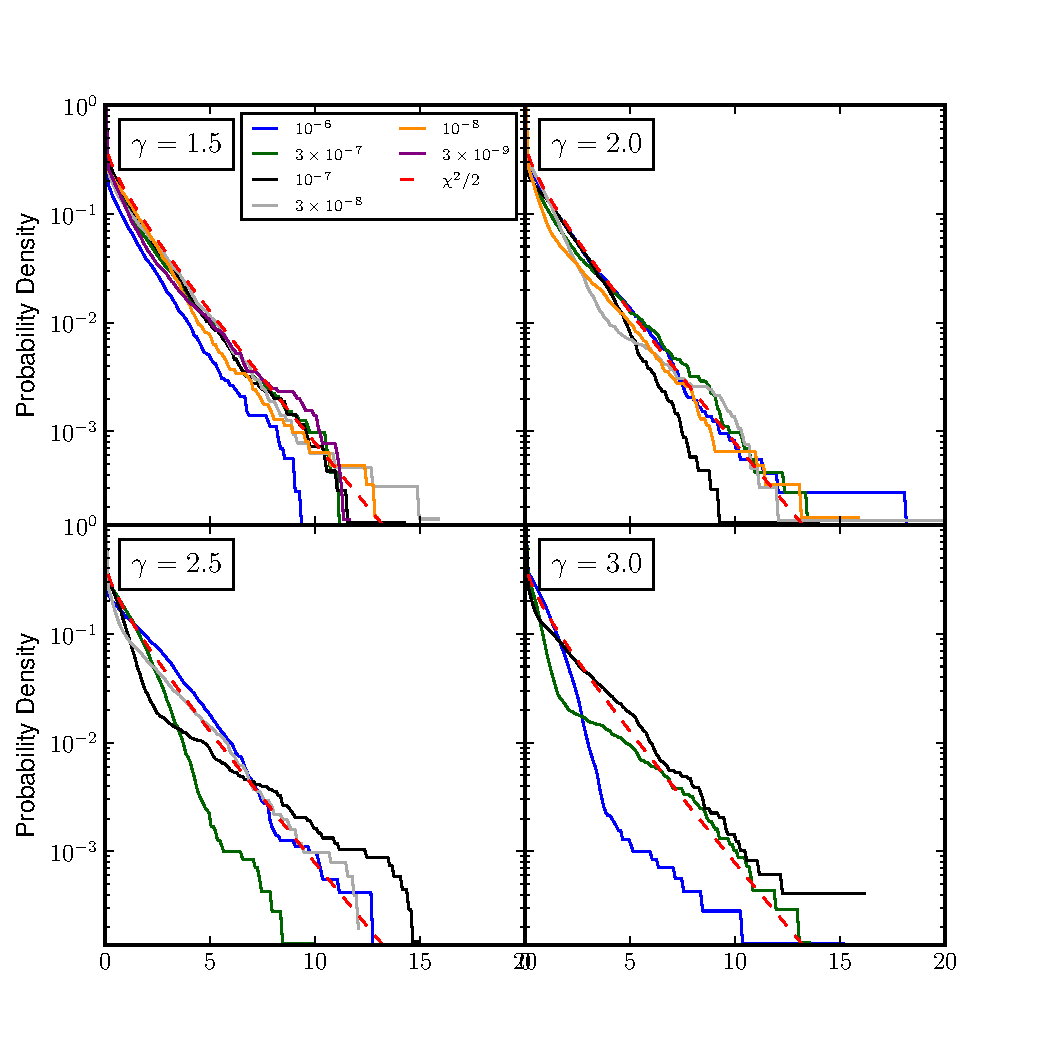
\includegraphics{mc_plots/ts_ext_emin_1000.pdf}
    % this plot came from /u/gl/lande/work/fermi/extended_catalog/monte_carlo/ts_ext/v3/plot.py
    % using data from /nfs/slac/g/ki/ki03/lande/extended_catalog/monte_carlo/ts_ext/v3_emin_1000/merged.hdf5
    \end{center}
    \caption{
    The results of the monte carlo simulation described in section
    \ref{monte_carlo_validation} testing the null distribution of
    the likelihood ratio test for extension.  The $x$ axis of this
    plot is \tsext and the $y$ axis is the cumulative density for
    \tsext that was found by testing simulated point sources of
    various spectral models for extension. The four plots represent
    different spectral indices (for $\gamma$ of 1, 2, 2.5, and 3).
    And the different colors lines represent different fluxes chosen
    to span a representative range of Overlayed on the plot in dashed
    red is the cumulative density function of $\chi^2(\ts)/2$ which is
    suggested by Wilk's theorem as the theoretical distribution these
    curves should should follow.  Overall, it should be noted that there
    is a surprisingly good agreement between the monte carlo study and
    the theoeretical distribution. And for most spectral parameters, the
    Monte Carlo curve lies to the left of the theoretical curve, which
    would imply that using Wilk's Theorem as the null distribution would
    conservativly underestimate the signifcance of a source detection. In
    the rest of the paper, we use this theoretical curve to estimate
    the significance of our source detections.  What is quoted is the
    $>100\mev$ integral flux in measured in units of $\ph/\cm^2/\s$.
    For each spectral model, more information about the simulations is
    summarized in table~\ref{ts_ext_num_sims}.
    }\label{ts_ext_mc}
  \end{figure}

\clearpage

\begin{figure}
  \begin{center}
    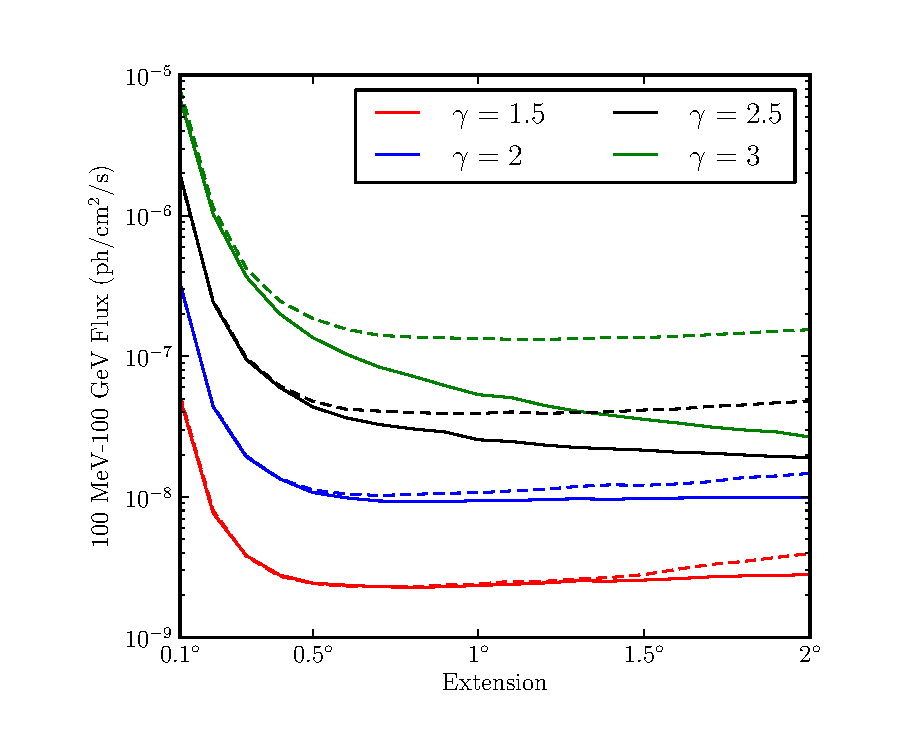
\includegraphics{mc_plots/index_sensitivity.pdf}
    % this plot came from /u/gl/lande/work/fermi/extended_catalog/monte_carlo/sensitivity/v9/plot_vs_index.py
    \end{center}
    \caption{Lalla}\label{index_sensitivity}
  \end{figure}

\clearpage

\begin{figure}
  \begin{center}
    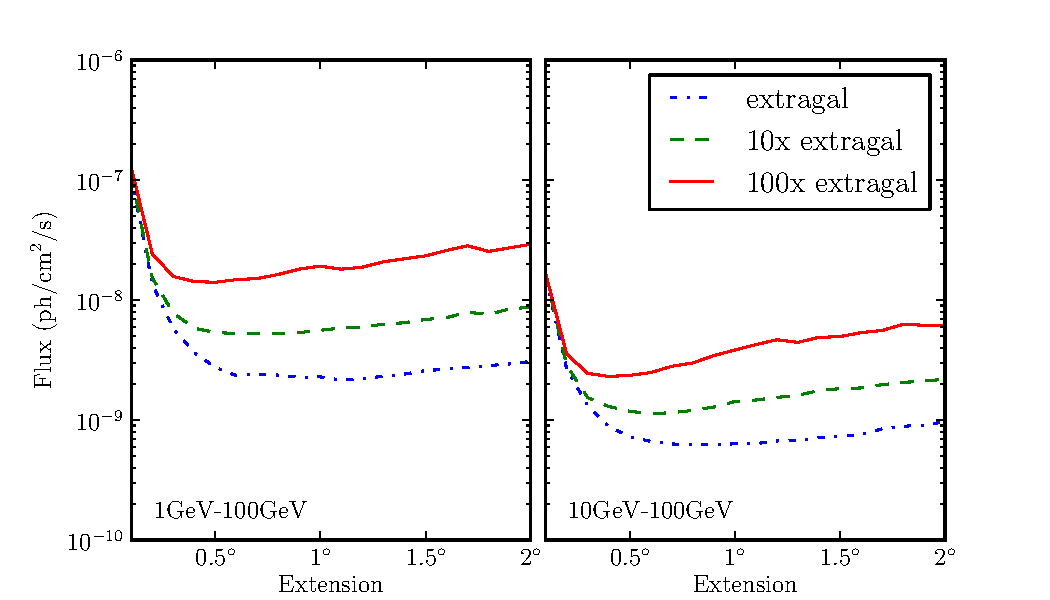
\includegraphics{mc_plots/diff_factor_sensitivity.pdf}
    % this plot came from /u/gl/lande/work/fermi/extended_catalog/monte_carlo/sensitivity/v9/plot_vs_diff_factor.py
    \end{center}
    \caption{Lalla}\label{diff_factor_sensitivity}
  \end{figure}

\begin{figure}
  \begin{center}
    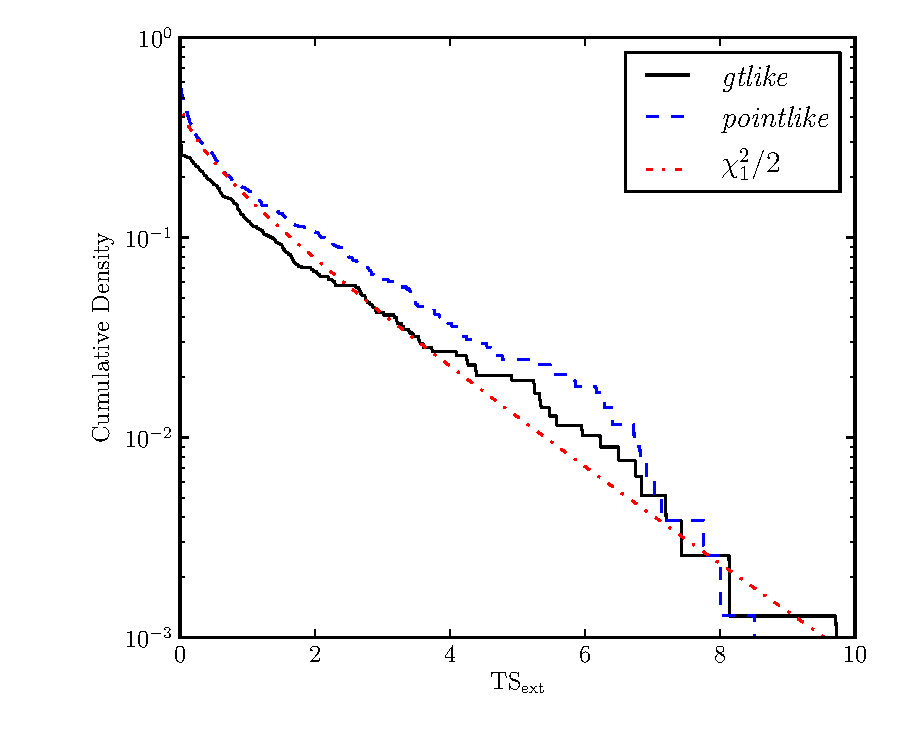
\includegraphics{source_plots/agn.pdf}
    % this plot came from /u/gl/lande/work/fermi/extended_catalog/2FGL/agn/v2/agn.py
    \end{center}
    \caption{Lalla}\label{agn_ts_ext}
  \end{figure}


\begin{figure}
  \begin{center}
  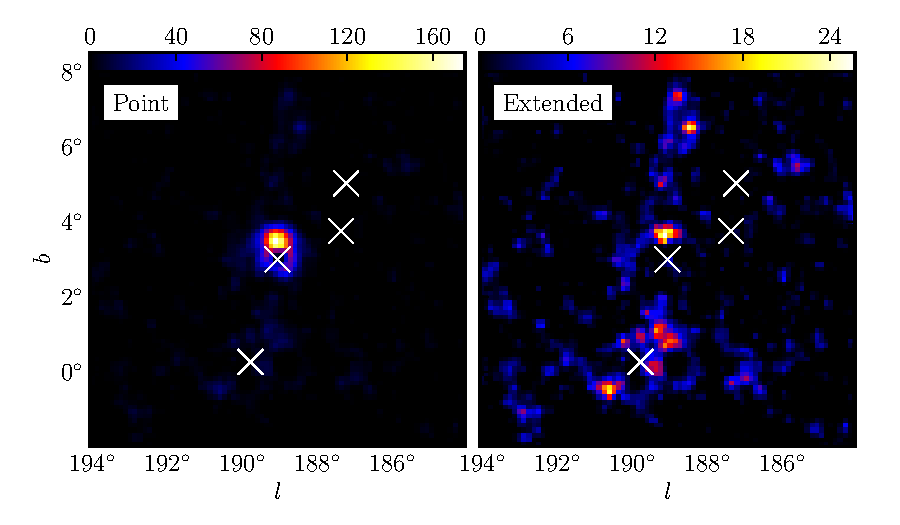
\includegraphics{ic443_plots/res_tsmap_ic443.pdf}
  % plot from /u/gl/lande/work/fermi/extended_catalog/2FGL/plots_for_paper/res_tsmap_ic443/v1

  \caption{An example residual test statistic map generated for the
  supernova rememnant IC443 using events between $1\gev$ and
  $100\gev$.  The top plot is the residual TS map fitting IC443
  as a point source and the bottom plot is the residual TS map fitting
  IC443 as an extended source. The crosses in the plot represent all of
  the sources fit in the region. Since there is a residual TS greater
  than 160 fitting with the point hypothesis, it is clear that a point
  source is not a good fit to the region. On the other hand,
  the residual TS fitting as an extended source is much lower, showing
  that IC443 is better fit by an extended source. These plots were generated
  for all extended source candidates to help validate the analysis.}
  \label{res_tsmaps}
  \end{center}
\end{figure}

\clearpage
\begin{figure}
  \begin{center}
    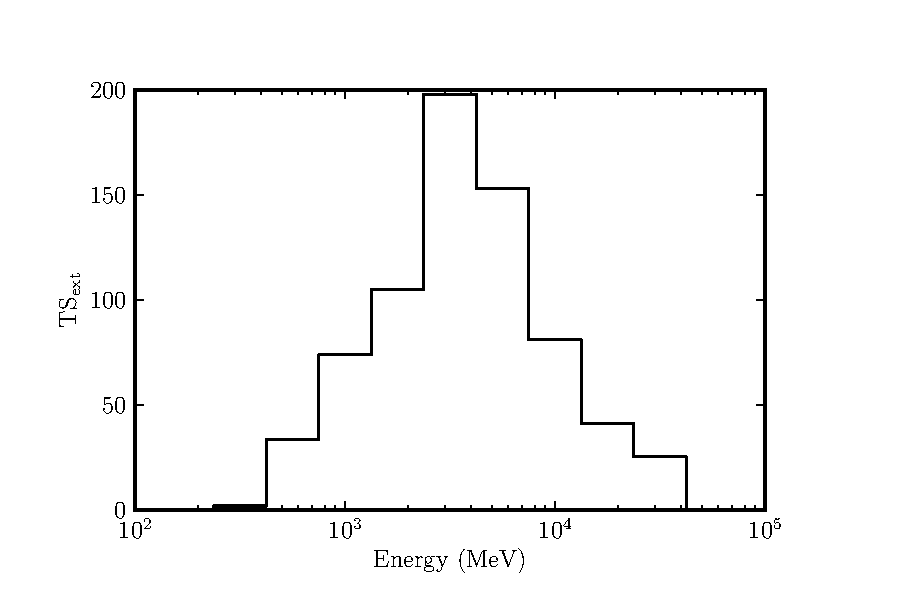
\includegraphics{ic443_plots/ic443_ts_ext_vs_energy.pdf}
    % taken from /u/gl/lande/work/fermi/extended_catalog/2FGL/plots_for_paper/ts_ext_vs_energy/v1/ts_ext_vs_energy.py
    \caption{\tsext vs log(energy)}
    \label{counts_slice}
  \end{center}
\end{figure}

\clearpage
\begin{figure}
  \begin{center}
    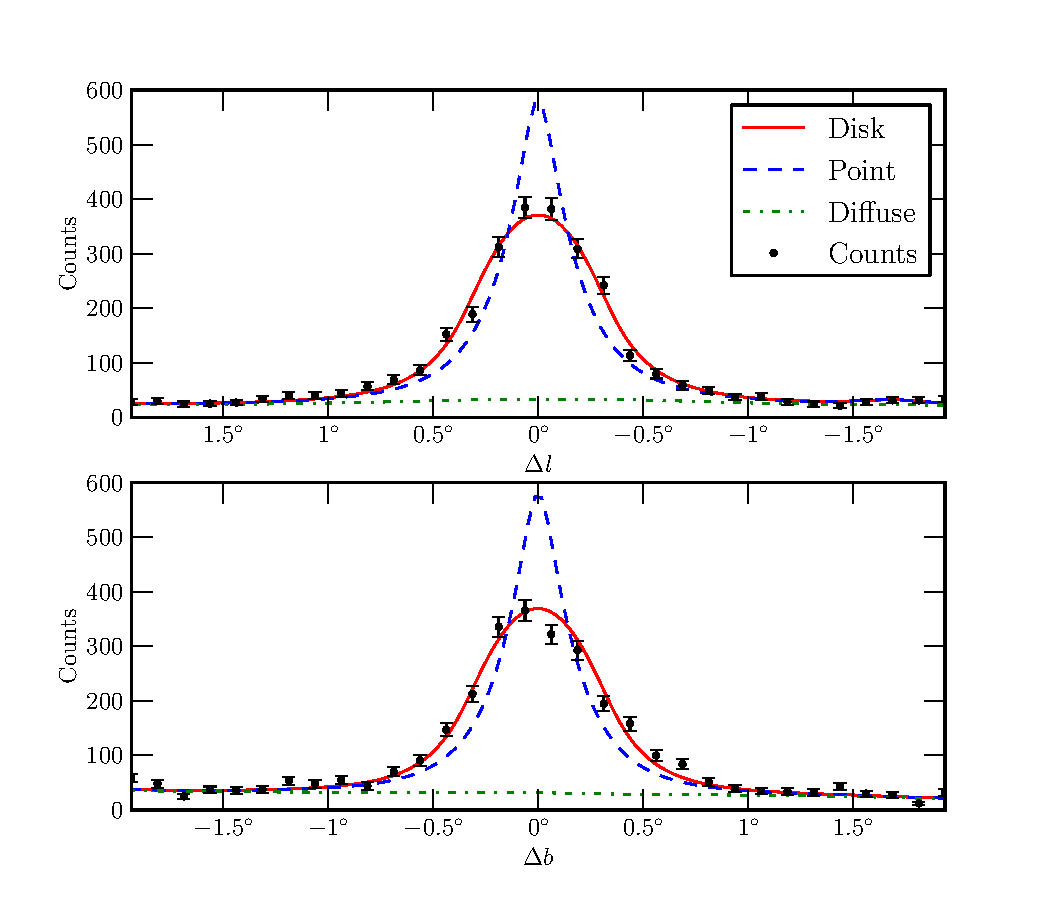
\includegraphics{ic443_plots/ic443_counts_slice.pdf}
    % taken from /u/gl/lande/work/fermi/extended_catalog/2FGL/plots_for_paper/counts_slice_ic443/v1/ic443_counts_slice.pdf
    \caption{Counts slice}
    \label{counts_slice}
  \end{center}
\end{figure}

\clearpage
\begin{figure}
  \begin{center}
    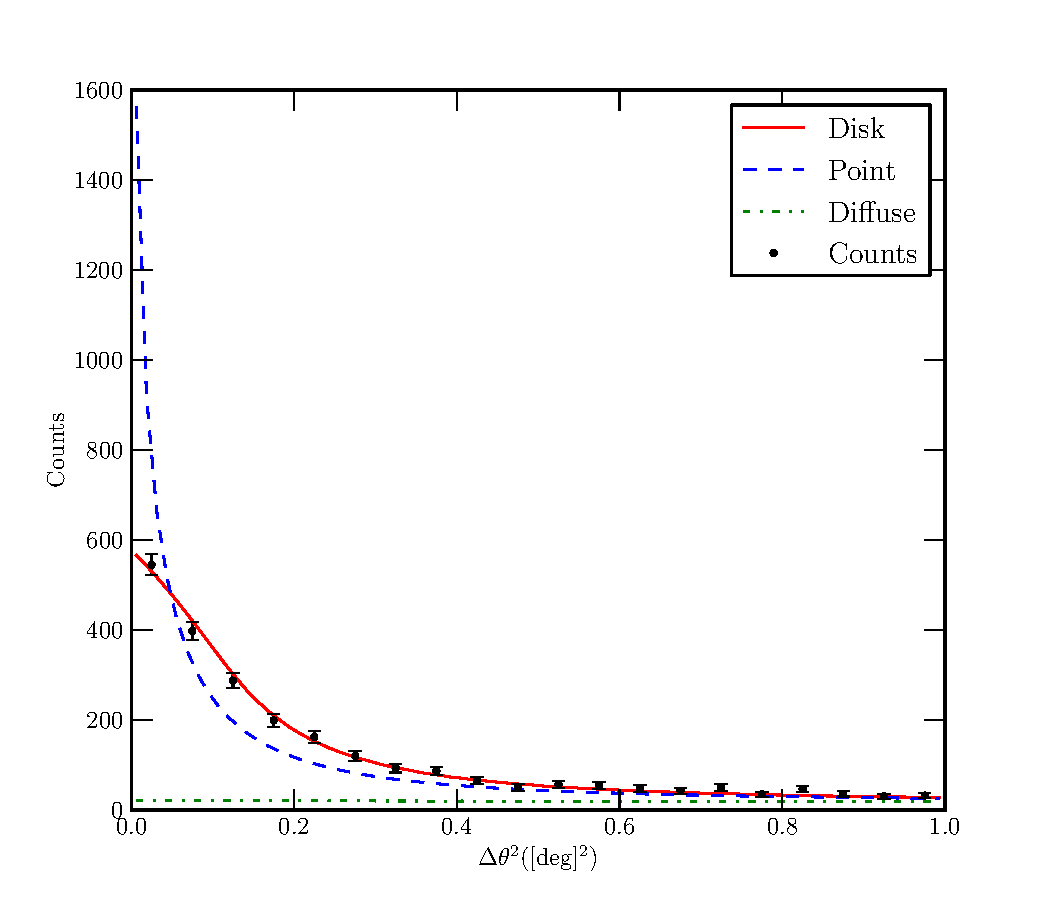
\includegraphics{ic443_plots/ic443_radial_integral.pdf}
    % taken from /u/gl/lande/work/fermi/extended_catalog/2FGL/plots_for_paper/radial_integral_ic443/v1/ic443_radial_integral.pdf
    \caption{The radial integral of the counts and the model predicted counts.}
    \label{radial_profile}
  \end{center}
\end{figure}

\clearpage
\begin{figure}
  \begin{center}
    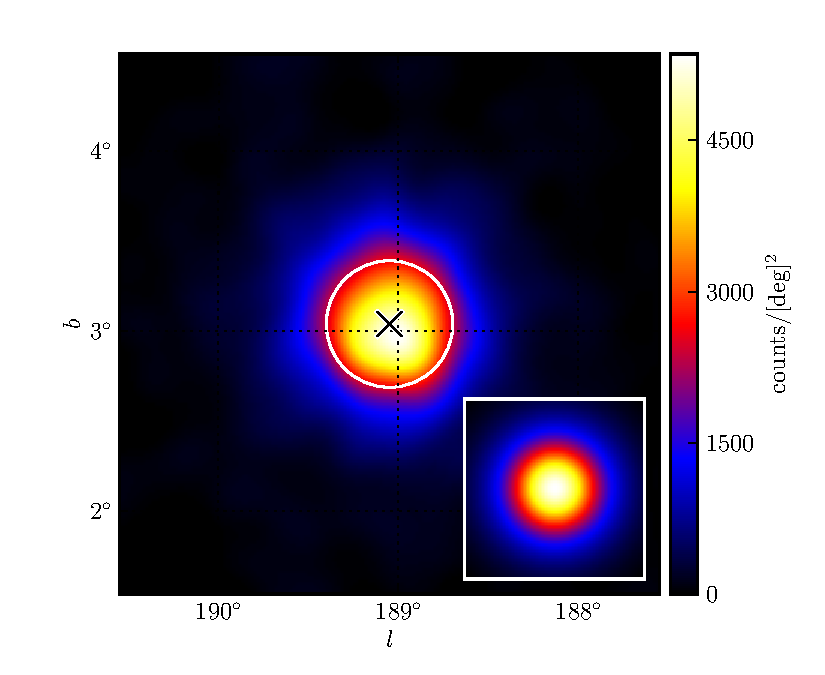
\includegraphics{ic443_plots/ic443_smoothed_counts.pdf}
    % taken from /u/gl/lande/work/fermi/extended_catalog/2FGL/plots_for_paper/smoothed_counts_ic443/v1
    \caption{Smoothed counts}
    \label{smoothed_counts}
  \end{center}
\end{figure}

\clearpage
\begin{sidewaystable}
    \begin{centering}
      \begin{tabular}{rrrrrrrrrrr}
        Name           &    GLON &    GLAT & $\sigma(^\circ)$ &     \ts & $\tsext$ & Major & Minor &   Ang & Flux ($10^{-9}$) &         Index \\
        \hline
        \multicolumn{11}{l}{$E > 1\gev$} \\
        \hline
        SMC            & 302.87  &  -44.65 &    $1.59\pm0.15$ &    93.1 &                   51.2 & 0.173 & 0.129 &  41.9 &   $3.0\pm0.4$    & $2.42\pm0.16$ \\
        LMC            & 278.58  &  -32.82 &    $2.26\pm0.09$ &   384.2 &                304.374 & 0.096 & 0.071 & -35.5 &  $12.9\pm0.7$    & $2.42\pm0.08$ \\
        IC443          & 189.05  &  3.04   &    $0.35\pm0.01$ & 10765.3 &                535.282 & 0.006 & 0.006 &  84.0 &  $65.2\pm1.2$    & $2.23\pm0.02$ \\
        W28            & 6.51    &  -0.29  &    $0.39\pm0.02$ &  1231.3 &                   92.1 & 0.014 & 0.013 &  30.4 &  $55.9\pm1.8$    & $2.65\pm0.03$ \\
        W30            & 8.61    &  -0.20  &    $0.36\pm0.04$ &   458.1 &                  66.0  & 0.020 & 0.018 &  14.1 &  $30.0\pm1.8$    & $2.58\pm0.06$ \\
        W44            & 34.68   &  -0.42  &    $0.34\pm0.02$ &  1387.6 &                  111.3 & 0.009 & 0.009 & -39.4 &  $74.7\pm1.0$    & $2.67\pm0.01$ \\
        W51C           & 49.12   &  -0.44  &    $0.28\pm0.02$ &  2174.7 &                   87.6 & 0.010 & 0.010 &  59.4 &  $41.6\pm1.3$    & $2.38\pm0.04$ \\
        \hline
        \multicolumn{11}{l}{$E > 10\gev$} \\
        \hline
        HESS J1825-137 &   17.58 &   -0.46 &    $0.64\pm0.08$ &    85.6 &                   62.5 & 0.050 & 0.045 & 33.6  &     $19.4\pm1.4$ & $2.27\pm0.07$ \\
        MSH 15-52      &  320.39 &   -1.22 &    $0.20\pm0.06$ &    73.7 &                    9.5 & 0.033 & 0.032 & 3.9   &      $4.7\pm0.7$ & $1.88\pm0.12$ \\
      \label{known_extended_sources}
      \end{tabular}
      \caption{The fit results for the known extended sources that
      were found by our analysis. The top results were found using
      an energy range between $1\gev$ and $100\gev$.
      The quoted flux is in units of $10^{-9}\ph/\cm^2/\s$ and 
      is the flux in the fit energy range.
      The lower analysis was done using events between
      $10\gev$ and $100\gev$ and the quoted flux
      values are in the fit energy range. All sources were
      fit using a disk morphology. The localiztaion and extension
      were found using \pointlike while the TS and spectral
      values were calculated using \gtlike.
      The TS value was computed using 
      the assumed disk morphology. The Centaurus A Lobes,
      the Cygnus Loop, and Vela X were not found to be extended by
      this too. The reasons for this are discussed in~\ref{validate_known}.
      }
    \end{centering}
\end{sidewaystable}


\clearpage

\begin{sidewaystable}
    \begin{centering}
      \begin{tabular}{rrrrrrrrrrr}
        Name           &    GLON &    GLAT & $\sigma(^\circ)$ &      TS & $\tsext$ & Major & Minor & Ang & Flux ($10^{-9}$) & Index \\
        \hline
        \multicolumn{11}{l}{$E > 1\gev$} \\
        \hline
        1FGL J1628.6-2419c \\
        1FGL J1554.0-5345c \\
        1FGL J0823.3-4248 \\
        \hline
        \multicolumn{11}{l}{$E > 10\gev$} \\
        \hline
        1FGL J2020.0+4049 \\
        1FGL J1837.5-0659c \\
        1FGL J1632.9-4802c \\
        1FGL J1613.6-5100c \\
        \hline
      \label{new_ext_srcs}
      \end{tabular}
      \caption{}
    \end{centering}
\end{sidewaystable}


  \begin{figure}
    \begin{center}
      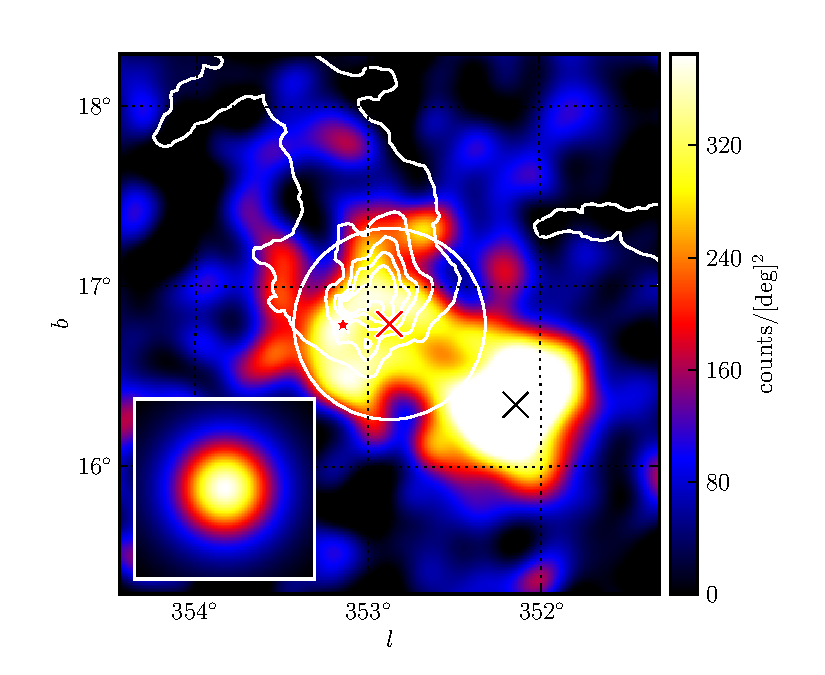
\includegraphics[type=pdf,ext=.pdf,read=.pdf]{source_plots/source_1FGL_J1628.6-2419c}
    \end{center}
    % this plot came from 
    % /nfs/slac/g/ki/ki03/lande/extended_catalog/2FGL/v10/spectral_emin_1000_v1/1FGL_J1628.6-2419c/v2/source_1FGL_J1628.6-2419c.pdf
    \caption{1FGL J1628.6-2419c}
  \end{figure}

  \begin{figure}
    \begin{center}
      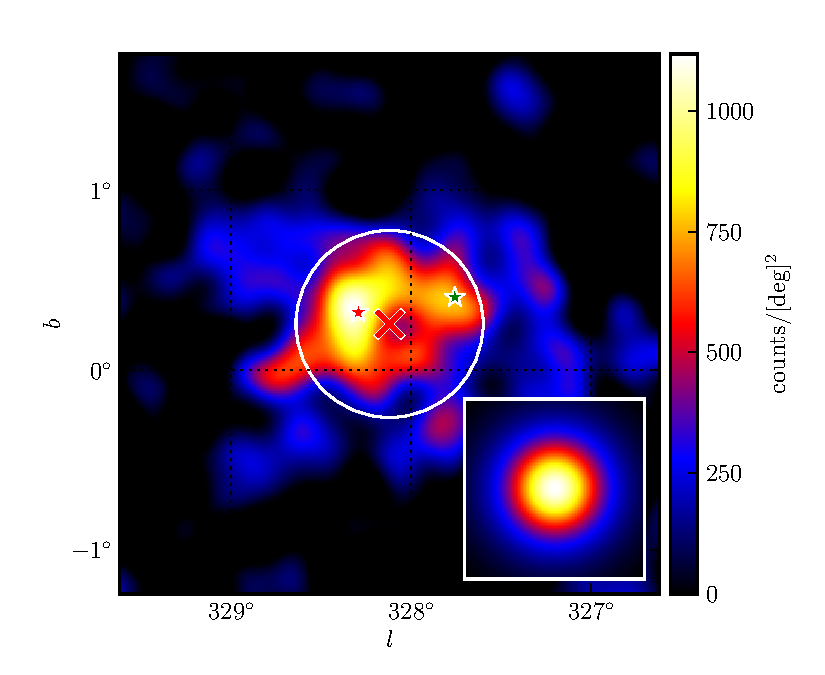
\includegraphics[type=pdf,ext=.pdf,read=.pdf]{source_plots/source_1FGL_J1554.0-5345c}
    \end{center}
    % this plot came from 
    % /nfs/slac/g/ki/ki03/lande/extended_catalog/2FGL/v10/spectral_emin_1000_v1/1FGL_J1554.0-5345c/v2/source_1FGL_J1554.0-5345c.pdf
    \caption{1FGL J1554.0-5345c}
  \end{figure}

  \begin{figure}
    \begin{center}
      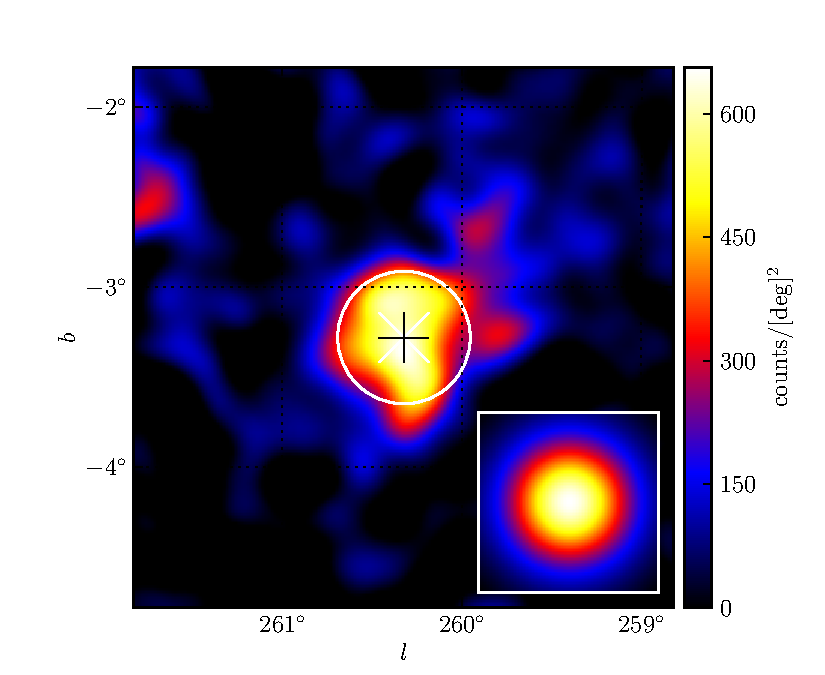
\includegraphics[type=pdf,ext=.pdf,read=.pdf]{source_plots/source_1FGL_J0823.3-4248}
    \end{center}
    % this plot came from 
    % /nfs/slac/g/ki/ki03/lande/extended_catalog/2FGL/v10/spectral_emin_1000_v1/1FGL_J0823.3-4248/v2/source_1FGL_J0823.3-4248.pdf
    \caption{1FGL J0823.3-4248}
  \end{figure}

  \begin{figure}
    \begin{center}
      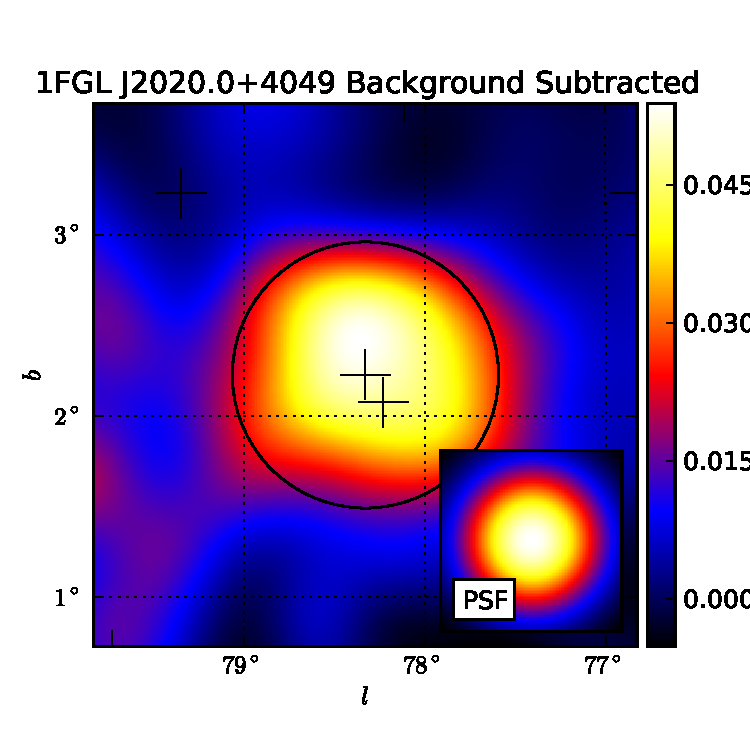
\includegraphics[type=pdf,ext=.pdf,read=.pdf]{source_plots/source_1FGL_J2020.0+4049}
    \end{center}
    % this plot came from 
    % /nfs/slac/g/ki/ki03/lande/extended_catalog/2FGL/v10/spectral_emin_10000_v1/1FGL_J2020.0+4049/v2/source_1FGL_J2020.0+4049.pdf
    \caption{
    1FGL J2020.0+4049
    }
  \end{figure}

  \begin{figure}
    \begin{center}
      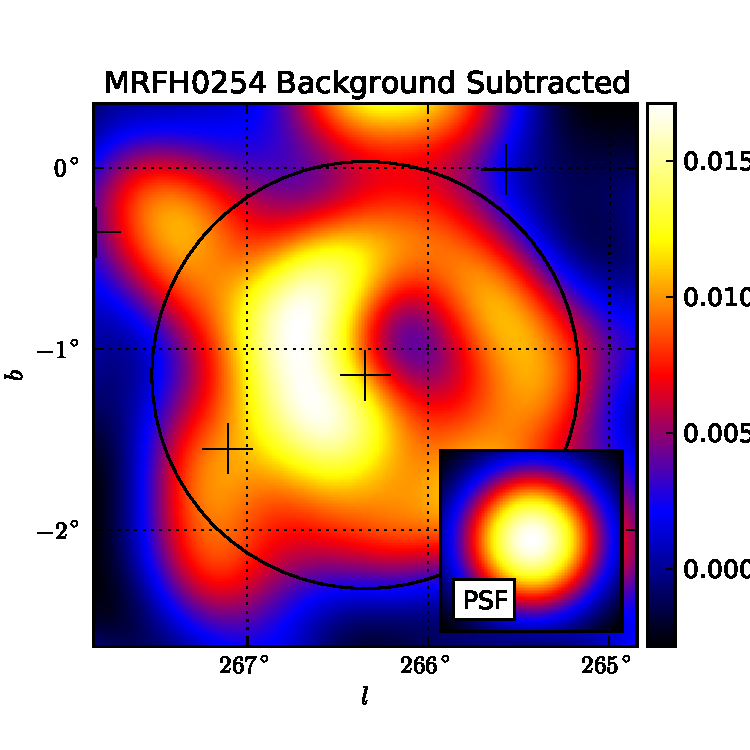
\includegraphics[type=pdf,ext=.pdf,read=.pdf]{source_plots/source_MRFH0254}
    \end{center}
    % this plot came from 
    % /nfs/slac/g/ki/ki03/lande/extended_catalog/2FGL/v10/spectral_emin_10000_v1/MRFH0254/v2/source_MRFH0254.pdf
    \caption{Lalla}
  \end{figure}

  \begin{figure}
    \begin{center}
      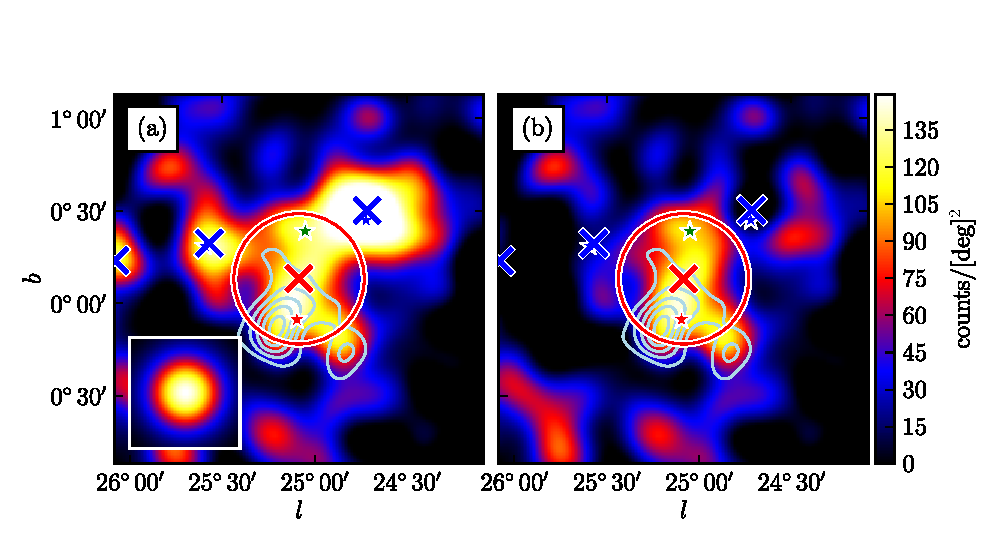
\includegraphics[type=pdf,ext=.pdf,read=.pdf]{source_plots/source_1FGL_J1837.5-0659c}
    \end{center}
    % this plot came from 
    % /nfs/slac/g/ki/ki03/lande/extended_catalog/2FGL/v10/spectral_emin_10000_v1/1FGL_J1837.5-0659c/v2/source_1FGL_J1837.5-0659c.pdf
    \caption{1FGL J1837.5-0659c}
  \end{figure}


  \begin{figure}
    \begin{center}
      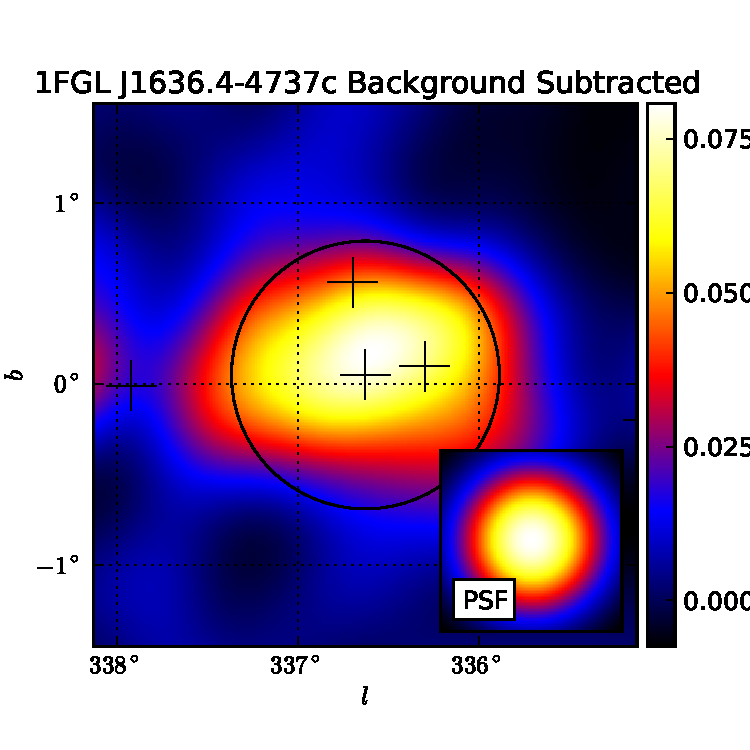
\includegraphics[type=pdf,ext=.pdf,read=.pdf]{source_plots/source_1FGL_J1636.4-4737c}
    \end{center}
    % this plot came from 
    % /nfs/slac/g/ki/ki03/lande/extended_catalog/2FGL/v10/spectral_emin_10000_v1/1FGL_J1636.4-4737c/v2/source_1FGL_J1636.4-4737c.pdf
    \caption{1FGL J1636.4-4737c}
  \end{figure}


  \begin{figure}
    \begin{center}
      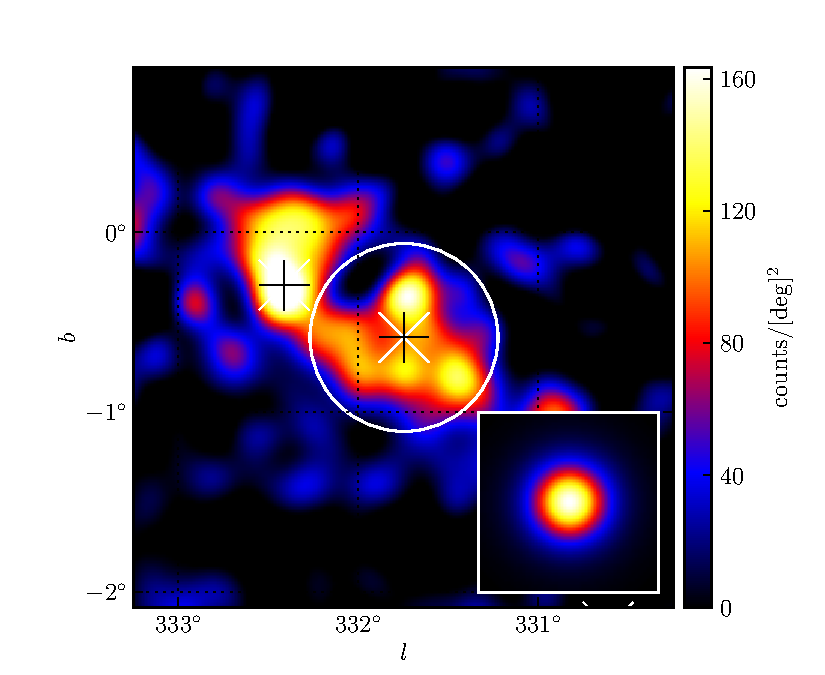
\includegraphics[type=pdf,ext=.pdf,read=.pdf]{source_plots/source_1FGL_J1613.6-5100c}
    \end{center}
    % this plot came from 
    % /nfs/slac/g/ki/ki03/lande/extended_catalog/2FGL/v10/spectral_emin_10000_v1/1FGL_J1613.6-5100c/v2/source_1FGL_J1613.6-5100c.pdf
    \caption{
    1FGL J1613.6-5100c }
  \end{figure}




  \end{document}

